\documentclass[main.tex]{subfiles}

\begin{document}

	\begingroup

	\renewcommand{\cleardoublepage}{}

	\renewcommand{\clearpage}{}

	\chapter{Clean Up Task Overview}

		\chapterauthor{Torge Olliges, Jan Schimpf}
		
		\section{Goal}
		The goal of the Clean Up task is like the name indicates to clean a room. In the RoboCup several objects get distributed through out the room. The objects can be placed on the floor, tables or other furniture. Each of these objects is clearly visible and not hidden behind something. The task of the HSR is now to find these objects and place them into an designated basket. There exist multiple target positions and the HSR has to decide by itself the correct one based on the object. Like the Storing Grocery task the time limit is 5 minutes.

	  	\section{Tasks}
	  	The figure \ref{clean_up_seq_01} shows the procedure of Clean Up. The following subsections explain the execution and procedure in detail and give insights into the decisions made resulting in the exact plan depicted below. Additionally a more in depth explanation of some of the challenges will be given 	

	  	\begin{figure}	
	  		\centering
	  		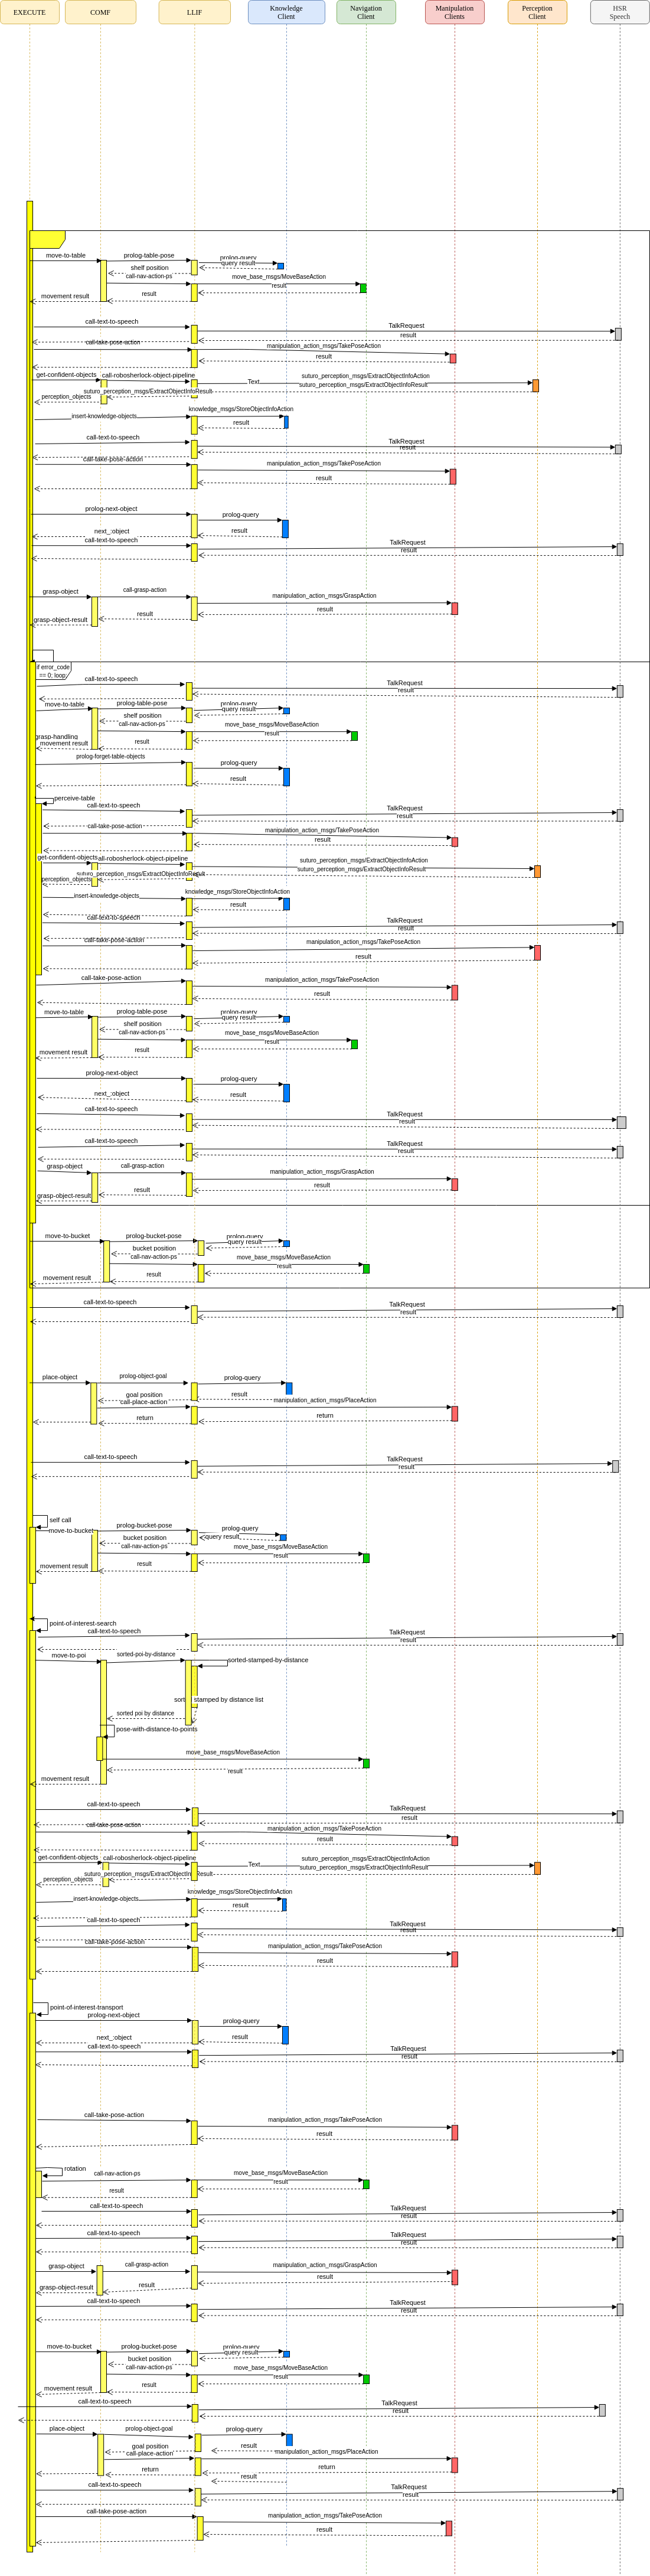
\includegraphics[width=0.85\textwidth]{pictures/diagramms/cleanup-sequence.png}
	  		\caption{Sequence diagram of the complete run of the clean up task \textit{(explanations below)}}
	  		\label{clean_up_seq_01}
	  	\end{figure}
	  	% TODO: Entfernen - hier bitte aus dem sequenz diagramm einen einzelnen task als subsection z.b. schritt: tür öffnen, dafür mussten perception dies tun manipulation das tun etc.
	  	
	\subsection{Setup}
	First the interface to Knowledge is called to set the \textit{target} to basket. In addition, the floor and the table are set as \textit{sources}, since objects are picked up from both. 

	\subsection{Scan table sequence}
	% Manipulation: take pose action
	The robot is set to the default pose to make sure it is in a neutral state. This is important in order to avoid moving the robot for example with an extended arm.
	
	% NLP: Talk Request	
	The talk requests are used to inform the developer as well as the people following the robot or evaluating its behavior about what the robot is about to do. They are also used for safety measures so the robot can warn when it is going to move so bystanders can step aside. 
	
	% Knowledge: get table-poses
	Knowledge finds all the tables available, sorts them by their distance to the robot and then returns the list of their position to Planning, so Planning can determine where to go next.
	
	% Navigation: moveBaseAction	
	The robot moves to the designated location in this case the table, it will be turned $90^\circ$ so it is in a pose where perceiving the table isn't hindered by the arm of the HSR. 
	
	% NLP
	Informing that the robot is perceiving the table now.
	
	% Manipuilation: TakePoseAction
	Manipulation gets the task to put the HSR into a pose to perceive an object depending on the height of the plane the object is on.
    That is necessary for Perception to get a good angle and distance to the object and to avoid having the robots arm block the cameras view.
	
	% Perception: Percieve and return data
	The HSR takes a picture of the scene it is currently looking at and processes it with \textit{RoboSherlock}. Based on the requested region the input images are filtered. The results are then published by the \textit{perception\_actionserver}.

	
	% Knowledge: Store Data
	Knowledge checks the data of the object, that is supposed to be stored. If the class is unknown to knowledge, it is set to other. If the data is valid the object gets added to the knowledge base and the objects at the position of the new object are put into a group.
	% NLP: Talk Request
	
	% Manipulation: Take pose
	The robot is set to the default pose.
	
	% 2x NLP: Talk
		
	% Navigation: MoveBaseAction
	Turn the HSR by $90^\circ$ so he can grasp objects which would not be possible from the pose he took to perceive the objects.
	
	\subsection{Grasp sequence}\label{clean_up_grasp_seq}
	
	%prolog-next-object
    The Knowledge base is queried for next Object that should be grasped.
	What the next object should be is determined by \textbf{KNOWLEDGE LEUTE MÜSSEN DAS ERKLÄREN}.	
	
	%NLP Grasping object
	Informing that the robot will now grasp an object
	%NLP Which object
	Informing which object the robot will grasp using the object id
	
	%grasp-object
	The object id is used to query the Knowledge base for the dimensions of the object and the pose of the object. The results are then used to call the manipulation grasp server to grasp the object. Manipulation then gets the task to grasp the given object. To do that the Grasp Action Server has to calculate the correct orientations to grasp from the right direction and do collision avoidance with all other objects which is done by using \textit{Giskard}.
	 %Knowledge: prolog dimensions
	 %Knowledge: prolog pose
	 
	%NLP succesfully grasped
	Informing that the robot has successfully grasped an object
    
	\subsection{Place sequence}
	%Navigation: moveBaseAction
	The robot moves to the designated location in this case the bucket.
	The coordinates for the navigation call are queried from the Knowledge base and adjusted so the robot looks at the bucket and can place the object inside it. 
	
	%NLP placing the object
	Informing that the robot is now placing the object

	%place-object
	The object id is used to query the Knowledge base for the dimensions of the object and the goal of the object. The results are then used to call the manipulation place server to place the object. Manipulation then gets the task to place the previously grasped object in the given destination. To do that the Place Action Server has to calculate the correct orientations to place from the right direction and do collision avoidance with all other objects which is done by using \textit{Giskard}.
	 %Knowledge: prolog dimensions
	 %Knowledge: prolog goal
	 
	%NLP placed the object
	Informing that the robot has successfully placed the object

	%Manipulation: Take pose
	Returns the robot into the default pose.
	
	This is looped for two times.
	The first one is for the table and stops if there are no more objects on it to be placed in the bucked. The sedon one is for the point of interest search and stops if there are not points of interest left.
	
	\subsection{Point of interest search sequence}
	The object finder node publishes a list of poses that may be an object. This list will from now on be called points of interests.
	
    %NLP found an point of interest to search
    Informing that the robot has found a point of interest to search for objects
    
    %move-to-poi
    The first pose of the points of interest is taken. A target position is calculated that enables the HSR to perceive the position. This target pose is then send to navigation and executed.
    
    %call-take-pose-action
    The HSR is brought into the perceive pose for the floor.
    
    %NLP perceiving the postition
    Informing that the robot is now perceiving the position
      
    %call-robosherlock-object-pipeline
	The HSR takes a picture of the scene it is currently looking at and processes it with \textit{RoboSherlock}. Based on the requested region the input images are filtered. The results are then published by the \textit{perception\_actionserver}.

    
    %Knowledge:insert-knowledge-objects
    Knowledge checks the data of the object, that is supposed to be stored. If the class is unknown to knowledge, it is set to other. If the data is valid the object gets added to the knowledge base and the objects at the position of the new object are put into a group.
    
    %call-take-pose-action
   	Returns the robot into the default pose to be able to grasp the object.

    % Navigation: MoveBaseAction
    Turn the HSR by $90^\circ$ so he can grasp objects which would not be possible from the pose he took to perceive the objects.

    The plan continues from the \ref{clean_up_grasp_seq}.
    
    
	\section{Conclusion}
	The outcome of the Clean Up task can be declared as successful, the robot was in a executable and working state for the third milestone demo. During those runs it achieved it's tasks like grasping the objects of the table or from the floor, transporting the objects and placing them in the basket.
	Even with the run being successfully completed the plan has similar problems to the Grocery Storing task with the magnet sensors and there are still potential issues as the way items on the floor are currently searched for involves the laser scanner so items that are to small to be picked up by the laser scanner won't be found by the robot.
	\endgroup

\end{document}
